\documentclass[12pt]{article}

\title{Research Computing Coursework Report}
\author{James Hughes}

\usepackage{amsmath}
\usepackage{listings}
\usepackage{url}
\usepackage{hyperref}
\usepackage{graphicx}

\lstdefinestyle{style1}{
    basicstyle=\ttfamily\footnotesize,
    breakatwhitespace=false,
    breaklines=true,
    captionpos=b,
    numbers=left,
    numbersep=5pt,
}
\lstset{style=style1}

\bibliographystyle{unsrt}

\begin{document}

\maketitle
\newpage

\section*{Introduction}

Sudoku is a type of simple puzzle, commonly found in the games pages of major UK newspapers.
`The Times' first featured a Sudoku in 2004, but the puzzle can be traced back to a series of popular U.S. puzzle books decades earlier, where it was given the title `Number Place'\cite{sudoku}.
For consistency, we propose the following definitions for the game, its rules, and related terms.

\begin{enumerate}
    \item A Sudoku puzzle consists of a $9\times9$ \textbf{grid} where the aim is to fill each of the 81 \textbf{cells} with a single-digit number from 1--9, according to certain rules.
    \item Each puzzle is differentiated by the \textbf{clues} given on the grid to begin with, which restricts the possible solutions. The empty cells (which we denote with a $0$ in the code) must be filled in.
    \item (\textbf{Row condition}) Each row of 9 cells must contain the digits 1--9 exactly once.
    \item (\textbf{Column condition}) Each column of 9 cells must contain the digits 1--9 exactly once.
    \item The grid can be tesselated by 9 square subsets of cells in a $3\times3$ arrangement; these are referred to as the \textbf{boxes}.
    \item (\textbf{Box condition}) Each box must contain the digits 1--9 exactly once.
    \item A grid is \textbf{valid} if its entries satisfy all of the rules above.
    \item A grid is \textbf{solved} if it is valid and contains no cells that are empty.
\end{enumerate}

It should be noted that the arrangement of clues for the starting grid can correspond to zero, one, or multiple solutions.
In 2012, it was proved exhaustively that it is not possible to specify a Sudoku puzzle which has a unique solution if there are less than 17 clues given on the starting grid\cite{17min}.
Therefore, Sudoku puzzles that start with this number of clues represent the `hardest', in the sense that they have the smallest ratio of number of valid solutions to number of all possible solutions.
Such puzzles are used later on to check that the code can handle the toughest cases in a reasonable time.

\section*{Algorithm Selection and Prototyping}

The solution implemented in this repository uses a mixture of `backtracking' and `using templates' \cite{wiki1}.
It is a brute-force method, which relies on the fact that the rules of Sudoku inherently limit the number of possible arrangements of any given digit into nine cells on the grid---such an arrangement is called a `template'.
Using a combinatorial argument, filling in the $3\times3$ boxes from left-to-right then top-to-bottom, we can see that there are 9 choices in the first box, then 6 choices and so on for a total of:
\[
    \text{Number of possible templates} = 9\cdot6\cdot3\cdot6\cdot4\cdot2\cdot4\cdot2\cdot1 = 46656.
\]
The method involves generating all such templates, and then finding the subset of templates that are valid in the context of each digit, with respect to the given clues.
Then, based on the remaining possibilities, we search through all possible combinations of entries of the empty cells using the `backtracking' approach.

The brute-force nature of the algorithm ensures robustness: whenever a solution exists it will always be found by the algorithm, as the entire space of solutions is searched.
In addition, brute-force has the advantage of a simple implementation, and is appropriate due to the relatively small size of the search space of even the hardest puzzles.
The use of templates decreases the size of the search space massively, and hence speeds up the algorithm so long as it is optimised.

The main concern in the initial development plan was how to store the collection of all template grids, and the sudoku grids themselves.
The use of the NumPy package enables these to be stored as \texttt{np.ndarray} types, enabling a large number of mathematical and logical operations to be performed on them at high speeds.
Moreover, assuming the default NumPy behaviour of storing integer arrays as 64-bit signed integers, the template collection would require $46656\cdot81\cdot8\approx3\cdot10^7$ bytes, or 30MB, of memory which is fine for any modern specification computer.
The development of the frontend code responsible for transforming these arrays to and from string or text formats would depend on the specific representation of the grids used in the solving algorithms.
Therefore the backend solving functionality was developed first.
It was appropriate for these two different parts of the codebase to be separated into two modules under the \texttt{sudokutools} package.
The final concern apparent before any development occurred was the need for subtle error catching, particularly in the case of puzzles with no solution, to avoid the program running indefinitely.

\section*{Development, Experimentation and Profiling}
The strategy for development was testing-led.
This meant that some of the earliest development steps was the creation of unit tests to ensure that the next anticipated phase of development was working properly.
This was done iteratively; as more functionality was developed, more tests were designed to guide the next phase of development, ensuring a defined development path throughout.
For instance, the following unit test was created in one of the earliest commits (\texttt{3132ebb}):

\begin{lstlisting}
    def test_templates():
    count_array = np.zeros((9, 9))
    for template_array in generate_templates():
        count_array += template_array
    count_array_expected = 5184 * np.ones((9, 9))
    assert count_array == count_array_expected
\end{lstlisting}

Tests like this one provide instant validation for the intended function, here \texttt{genera\_templates}, once it has been developed, and also specify the expected format of the inputs and outputs.

The repository was version controlled using Git.
Three branches were used: \texttt{main}, \texttt{dev}, and \texttt{test}.
The code was primarily developed in the \texttt{dev} branch, and then merged to main once the current testing suite was satisfied.
The \texttt{test} branch was intended for experimental features---namely any ideas that deviated strongly from the original plan.
The commit message style was strictly consistent for almost all commits, following the `Convential Commits' guidance \cite{ccommits}.
In particular, every commit had a regular structure, starting with one of a pre-defined list of `type' words suggested by \cite{ccommits}, such as `Fix' or `Docs'.
This is then followed by an imperative verb and then a full sentence, to informatively describe the changes made.

Development began with the backend functions \texttt{generate\_templates} and then \texttt{find\_valid\_templates}.
The former implemented a generator which iterated through all possible templates, where 0's represent empty cells and 1's represent the chosen digit.
The function does this by representing such a grid using a list of integers of length 9, where:
\begin{itemize}
    \item the $i^{th}$ digit of the list is the column to which the 1 in the $i^{th}$ row belongs - so the row condition holds;
    \item the column condition is satisfied by only iterating through permutations of (1,...,9); and,
    \item the box condition is satisfied by finding the remainder of each entry of the array when divided by 3, corresponding to the three boxes on that row, and checking the first, second and third group of 3 entries of the array are individually permutations of (0, 1, 2).
\end{itemize}

Regular refactoring was a crucial part of the development strategy.
For instance, the original implementation of \texttt{find\_valid\_templates} used a double-nested \texttt{for} loop to check each cell, and created a list of the other digits on each iteration, in order to check whether any of the 8 remaining digits' clues conflicted with a template.
In commit \texttt{60a4faa4}, this was then changed to initialise the list of \texttt{OTHER\_DIGITS} as a global variable in the module, so that it was only constructed once, saving computational time.
The nested for loops were also substituted for the use of the NumPy method \texttt{isin} which later became the use of NumPy's \texttt{any} method.
This refactoring not only improved the computational speed of the routine, but also achieved the same functionality in fewer lines, improving readability of the code.

The next major step was implementing the final solving function.
The first prototype of this algortihm used a simple \texttt{for} loop to iterate through the Cartesian product of the subsets of templates for each digit.
This was tried before the backtracking algorithm since it only required a very short (11 lines), readable routine, and was therefore worth investigating to see if it was viable.
This passed the testing suite, but was immediately found to be very slow for any non-trivial starting grid.

At this point, considering how one would solve some of the hardest Sudoku grids by hand illuminated the fact that a further `smart' filtering step of the subsets of templates was possible.
In particular, in some cases the initial clues for a given digit allow certain cells to be filled immediately by using the fact that they are a kind of 'fixed point' in the subset of templates, that is, in all valid templates, a certain cell is always occupied by that digit, but this isn't given as an explicit clue.
The simplest case of this is when, say, there are 8 clues for the digit 1, meaning that there is a 9th cell that must also be occupied by a 1.
This experimental feature was developed in the \texttt{refine\_valid\_templates} method in the \texttt{test} branch, which fills in any such cells and then calls \texttt{find\_valid\_templates} again, in a loop.
This feature uses a brute-force style approach, but in each instance the search space is very small---it is just the subset of valid templates for some digit.
In some of the starting grids with more clues, this routine was found to be sufficient to solve the grid entirely.

After this, it was clear that the proper backtracking part of the solving algorithm was necessary to solve---in a reasonable time-frame---the grids that were still fairly empty after the new template step.
In the first prototype of this routine, a nested list (with a $9\times9$ shape) of generators was instantiated in the beginning, with each generator representing the possible digits that could occupy the corresponding cell.
A NumPy array \texttt{search\_positions} was used to store the coordinates of the cells that were empty, i.e. the cells that were involved in the search.
The variable \texttt{search\_idx} was initialised at zero, and used to keep track of the current location of the backtracking procedure on the grid.
The backtracking routine then loops through the following steps:
\begin{enumerate}
    \item Try the next possible digit in the current cell.
    \item If the current grid is now valid, increase \texttt{search\_idx} by 1. Otherwise, revert to the first possible digit and decrease by 1.
    \item If \texttt{search\_idx} reaches the index of the last `empty' cell and the grid is solved, stop.
\end{enumerate}

Next, the data handling part of the code package was developed with two functions, \texttt{read\_grid} and \texttt{write\_grid}.
Their development began with simple prototypes that effectively handled the valid input cases.
Extensive error catching was then implemented.
It was appropriate to apply this to \texttt{sudokutools.data} first as this module contains front-end functions where the input is from a user, and is more susceptible to unexpected violations such as:
\begin{itemize}
    \item Formatting the grid incorrectly
    \item Not passing a .txt file.
    \item Specifying a non-existing file.
\end{itemize}
A lenient approach was taken in the case of a badly formatted grid; so long as the text file contained exactly 9 lines that contained any number of digit characters, and each of these contained exactly 9 digit characters, the input file was accepted.
This meant that any bad formatting involving non-numeric `decorating' characters was ignored, and also reduced the complexity of the code.
In the case of any of the other violations above, an informative string was printed explaining the error, and a grid containg negative entries was returned.

Following initial development, testing, and documentation, the next step was to profile the code using \texttt{line\_profiler}, whose outputs were exported as .txt files in a separate \texttt{prof} directory.
The function \texttt{solve\_backtrack} was profiled with input grids of varying difficulty, since this function also called all of the other backend solving functions.
Regardless of the starting grid, it was found that the largest percentage (between 75.5\% and 99.5\%) of runtime was spent calling the \texttt{find\_valid\_templates} and \texttt{refine\_valid\_templates} functions.
Further profiling revealed that the former function (which is used repeatedly by the latter) was the main bottleneck for computational time.

In order to optimise \texttt{find\_valid\_templates}, the full space of templates was represented as a 3D NumPy array of shape \texttt{(46656, 9, 9)} rather than as a list of arrays.
Similarly, where before the subsets of valid templates for each digit were stored in a nested list, this was also changed to be a NumPy array of shape \texttt{(9, 46656)}, with each row representing the indices of valid templates for that digit.
This enabled the use of NumPy's \texttt{any} method; rather than looping through the list of all templates, to find the list of valid templates.
This was compatible with the representation of the grid as a 2D NumPy array itself; the check now involved creating two new \texttt{(9, 9)} shaped arrays, representing the locations of the digit of interest, and the other digits in the grid, and then checking that both were compatible with the any given template array by using the \text{any} method across the 2nd and 3rd axes of the \texttt{ALL\_TEMPLATES} array.

\section*{Validation, Unit Tests and Continuous Integration}

The main form of continuous integration used in this project was via the\texttt{pre\-commit} package \cite{precommit}.
In this project, \texttt{Black} \cite{black} and \texttt{Flake8} \cite{flake8} were used, as well as some pre-defined hooks from the \texttt{pre-commit} repository itself.
The hooks imported from \texttt{pre-commit} apply simple checks to all file types, for instance checking that all files have a consistent newline character.
\texttt{Black} is a code formatter, which applies changes to files directly, usually rearranging code so that lines are not too long.
On the other hand, \texttt{Flake8} is a linter which means it only detects changes, but this typically allows it to be more stringent---for this reason it was made to be the final pre-commit hook, so that it could double check the changes made by \texttt{Black}.
\texttt{Black} and \texttt{Flake8} only apply to Python scripts, ensuring their compliance to PEP 8 \cite{pep8}, a widely-used style guide for Python.
However, these hooks were in conflict with eachother in certain instances.
For example, in trying to commit an updated \texttt{solve.py} script, \texttt{Black} was formatting a block of code to look like the following:
\begin{lstlisting}
    BOX_GRIDS[
        grid_idx,
        3 * (grid_idx // 3) : 3 * (grid_idx // 3) + 3,
        3 * (grid_idx % 3) : 3 * (grid_idx % 3) + 3,
    ] = 1
\end{lstlisting}
However, \texttt{Flake8} then blocked the commit, despite PEP 8 allowing spaces around colons when slicing\cite{wspace}.
Modifying the \texttt{Flake8} hook to include \texttt{args: [--extend-ignore=E203]} resolved this conflict; \texttt{Black}'s hook was changed to enforce line-lengths of 79 characters for a similar conflict resolution.
Notably, no hook was included to run the test-suite upon each commit, due to the long time taken for the test suite to run, particularly in the early stages of development.
An ideal project would include automatic running of the test suite upon any attempted merge to the main branch on the remote GitLab repository, and block such a merge if any test failed.

Due to the long testing times, the test-suite was split into multiple files so that subsets of the suite could be selected and run individually.
Each function had at least one test checking that it executed properly when passed the expected input.
Extra tests were then implemented to check that errors were caught properly, especially in the case of the frontend \texttt{data} functions as described previously.
The main case of error catching which is checked in the \texttt{solve} module is for the \texttt{solve\_backtrack} function whose input \texttt{grid} should be verified to ensure that the grid indeed has a solution.
There are three tests for this, including a grid that already contains invalid clues, and two subtler tests where the impossibility of the puzzles is harder to detect.

\begin{figure}[hbt]
    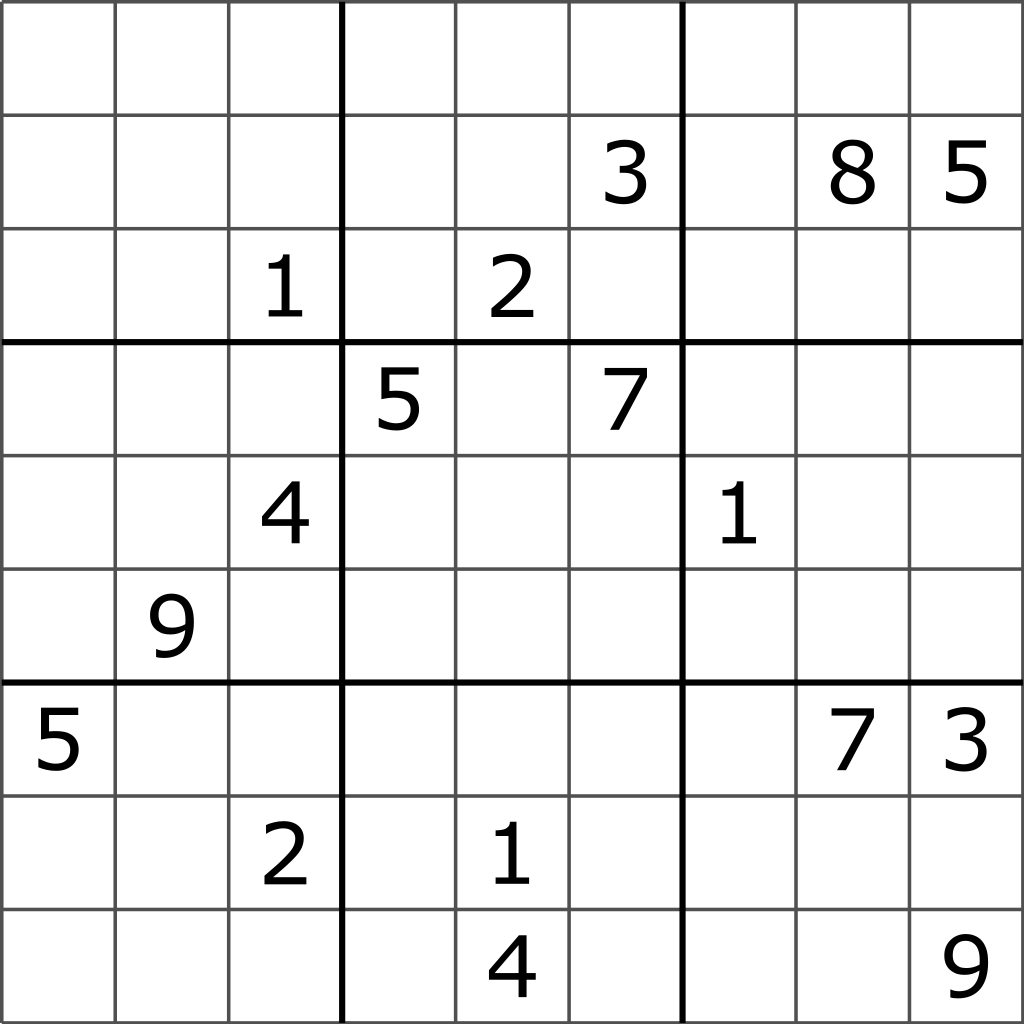
\includegraphics[scale=0.3]{Sudoku_puzzle_hard_for_brute_force.png}
    \caption{An antagonistically designed Sudoku puzzle. Note the digits in reverse order in the top row\cite{antagonist}.}
    \label{antagonist_clues}
\end{figure}

\section*{Packaging and Usability}

In the project Docker was used to make the code more portable.
A Dockerfile in the repository root directory specifies exactly how to build the Docker image, which starts with a basic image with conda already installed \cite{docker}.
It then builds the repository, and then updates the conda environment using \texttt{environment.yml}.
This file specifies the exact dependencies in the conda environment used to run the code, allowing for reproducible results.
It was exported from conda using the \texttt{--no-builds} option meaning that it can be used to reproduce the environment on any operating system.

The codebase was also documented using Doxygen \cite{doxygen}.
A frontpage gives an overview of the features of the repository, and there is documentation for every function and unit test.
The documentation is formatted as a .html page, with great readability and many hyperlinks between pages to see how some functions are connected.
In addition, the code itself is commented throughout.
The general approach was to focus on making code readable to the point of comments being unnecessary, with comments added sparsely at the end to explain complex blocks of code.

The documentation was improved by a consistent use of terminology and conventions, both in the plain language descriptions as well as variable, function, and module naming.
This makes it easy to keep track of the purpose of different parts of the code, especially when they are used in tandem.

\section*{Summary}

In summary, the task of developing Sudoku software is best tackled using sophisticated software development practices.
Without thorough use of the discussed techniques, all of the codebase could still have been produced, however it would have taken much longer, it would have contained more undetected bugs, and maintaining and sharing the project would have been much harder.
One example of this would be a bug fixed near the end of development, in commit \texttt{332a2dc}.
Before this change, the solving algorithm only caught impossible starting grids if their clues violated the rules, but ignored other subtler cases.
Since the code was well documented, and precise unit tests were implemented, it was easy to see exactly what error catching behaviours had been considered and validated in earlier development.
This enabled the bug to be spotted and fixed much more easily.

In a similar way, there is scope for further improvement. For instance, the algorithm could indicate the uniqueness of the solution, and even count the total number of possible solutions, or indicate if the clues constitue a `minimal' set of clues.
Due to the portability of the code, as well as the use of Git in sharing the repository, this task could easily be carried out by another developer completely new to the repository.

\bibliography{Biblio}

\end{document}
